% Graphic for TeX using PGF
% Title: /home/guillaume/Documents/Université de Montréal/Automne 2014/Génie logiciel/Devoir/devoir-3/diagramme-de-classes-changement-2.dia
% Creator: Dia v0.97.3
% CreationDate: Mon Dec  8 18:14:16 2014
% For: guillaume
% \usepackage{tikz}
% The following commands are not supported in PSTricks at present
% We define them conditionally, so when they are implemented,
% this pgf file will use them.
\ifx\du\undefined
  \newlength{\du}
\fi
\setlength{\du}{15\unitlength}
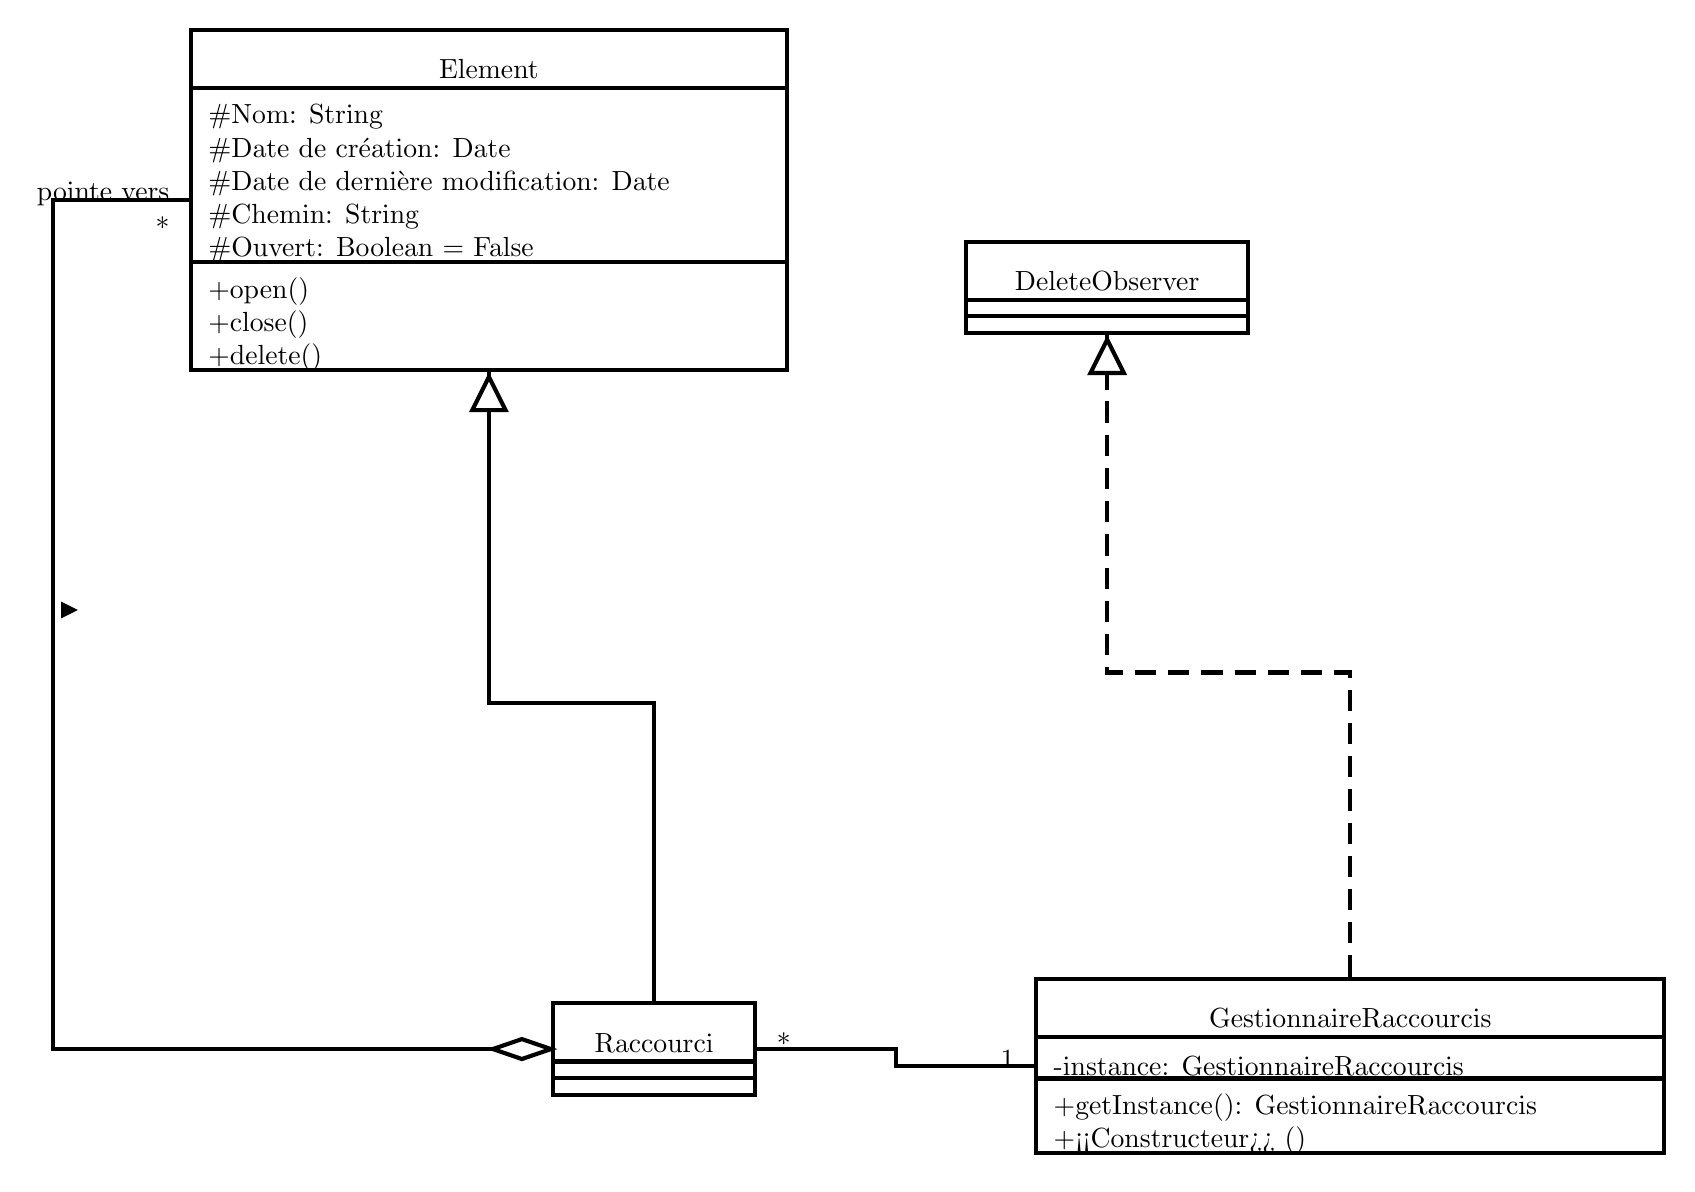
\begin{tikzpicture}
\pgftransformxscale{1.000000}
\pgftransformyscale{-1.000000}
\definecolor{dialinecolor}{rgb}{0.000000, 0.000000, 0.000000}
\pgfsetstrokecolor{dialinecolor}
\definecolor{dialinecolor}{rgb}{1.000000, 1.000000, 1.000000}
\pgfsetfillcolor{dialinecolor}
\pgfsetlinewidth{0.100000\du}
\pgfsetdash{}{0pt}
\definecolor{dialinecolor}{rgb}{1.000000, 1.000000, 1.000000}
\pgfsetfillcolor{dialinecolor}
\fill (13.909500\du,17.090000\du)--(13.909500\du,18.490000\du)--(18.779500\du,18.490000\du)--(18.779500\du,17.090000\du)--cycle;
\definecolor{dialinecolor}{rgb}{0.000000, 0.000000, 0.000000}
\pgfsetstrokecolor{dialinecolor}
\draw (13.909500\du,17.090000\du)--(13.909500\du,18.490000\du)--(18.779500\du,18.490000\du)--(18.779500\du,17.090000\du)--cycle;
% setfont left to latex
\definecolor{dialinecolor}{rgb}{0.000000, 0.000000, 0.000000}
\pgfsetstrokecolor{dialinecolor}
\node at (16.344500\du,18.040000\du){Raccourci};
\definecolor{dialinecolor}{rgb}{1.000000, 1.000000, 1.000000}
\pgfsetfillcolor{dialinecolor}
\fill (13.909500\du,18.490000\du)--(13.909500\du,18.890000\du)--(18.779500\du,18.890000\du)--(18.779500\du,18.490000\du)--cycle;
\definecolor{dialinecolor}{rgb}{0.000000, 0.000000, 0.000000}
\pgfsetstrokecolor{dialinecolor}
\draw (13.909500\du,18.490000\du)--(13.909500\du,18.890000\du)--(18.779500\du,18.890000\du)--(18.779500\du,18.490000\du)--cycle;
\definecolor{dialinecolor}{rgb}{1.000000, 1.000000, 1.000000}
\pgfsetfillcolor{dialinecolor}
\fill (13.909500\du,18.890000\du)--(13.909500\du,19.290000\du)--(18.779500\du,19.290000\du)--(18.779500\du,18.890000\du)--cycle;
\definecolor{dialinecolor}{rgb}{0.000000, 0.000000, 0.000000}
\pgfsetstrokecolor{dialinecolor}
\draw (13.909500\du,18.890000\du)--(13.909500\du,19.290000\du)--(18.779500\du,19.290000\du)--(18.779500\du,18.890000\du)--cycle;
\pgfsetlinewidth{0.100000\du}
\pgfsetdash{}{0pt}
\pgfsetmiterjoin
\pgfsetbuttcap
{
\definecolor{dialinecolor}{rgb}{0.000000, 0.000000, 0.000000}
\pgfsetfillcolor{dialinecolor}
% was here!!!
\definecolor{dialinecolor}{rgb}{0.000000, 0.000000, 0.000000}
\pgfsetstrokecolor{dialinecolor}
\draw (13.860710\du,18.190000\du)--(1.862500\du,18.190000\du)--(1.862500\du,-2.265000\du)--(5.139403\du,-2.265000\du);
}
\definecolor{dialinecolor}{rgb}{0.000000, 0.000000, 0.000000}
\pgfsetstrokecolor{dialinecolor}
\draw (12.602131\du,18.190000\du)--(1.862500\du,18.190000\du)--(1.862500\du,-2.265000\du)--(5.139403\du,-2.265000\du);
\pgfsetdash{}{0pt}
\pgfsetmiterjoin
\pgfsetbuttcap
\definecolor{dialinecolor}{rgb}{1.000000, 1.000000, 1.000000}
\pgfsetfillcolor{dialinecolor}
\fill (13.860710\du,18.190000\du)--(13.160710\du,18.430000\du)--(12.460710\du,18.190000\du)--(13.160710\du,17.950000\du)--cycle;
\pgfsetlinewidth{0.100000\du}
\pgfsetdash{}{0pt}
\pgfsetmiterjoin
\pgfsetbuttcap
\definecolor{dialinecolor}{rgb}{0.000000, 0.000000, 0.000000}
\pgfsetstrokecolor{dialinecolor}
\draw (13.860710\du,18.190000\du)--(13.160710\du,18.430000\du)--(12.460710\du,18.190000\du)--(13.160710\du,17.950000\du)--cycle;
% setfont left to latex
\definecolor{dialinecolor}{rgb}{0.000000, 0.000000, 0.000000}
\pgfsetstrokecolor{dialinecolor}
\node[anchor=west] at (1.962500\du,7.812500\du){};
\definecolor{dialinecolor}{rgb}{0.000000, 0.000000, 0.000000}
\pgfsetfillcolor{dialinecolor}
\fill (2.062500\du,7.812500\du)--(2.062500\du,7.412500\du)--(2.462500\du,7.612500\du)--cycle;
\definecolor{dialinecolor}{rgb}{0.000000, 0.000000, 0.000000}
\pgfsetstrokecolor{dialinecolor}
\node[anchor=east] at (12.260710\du,18.040000\du){};
\definecolor{dialinecolor}{rgb}{0.000000, 0.000000, 0.000000}
\pgfsetstrokecolor{dialinecolor}
\node[anchor=east] at (4.939403\du,-2.415000\du){ pointe vers};
\definecolor{dialinecolor}{rgb}{0.000000, 0.000000, 0.000000}
\pgfsetstrokecolor{dialinecolor}
\node[anchor=east] at (4.939403\du,-1.615000\du){*};
\pgfsetlinewidth{0.100000\du}
\pgfsetdash{}{0pt}
\pgfsetmiterjoin
\pgfsetbuttcap
{
\definecolor{dialinecolor}{rgb}{0.000000, 0.000000, 0.000000}
\pgfsetfillcolor{dialinecolor}
% was here!!!
\definecolor{dialinecolor}{rgb}{0.000000, 0.000000, 0.000000}
\pgfsetstrokecolor{dialinecolor}
\draw (12.365000\du,1.885253\du)--(12.365000\du,9.862486\du)--(16.344500\du,9.862486\du)--(16.344500\du,17.039719\du);
}
\definecolor{dialinecolor}{rgb}{0.000000, 0.000000, 0.000000}
\pgfsetstrokecolor{dialinecolor}
\draw (12.365000\du,2.797057\du)--(12.365000\du,9.862486\du)--(16.344500\du,9.862486\du)--(16.344500\du,17.039719\du);
\pgfsetmiterjoin
\definecolor{dialinecolor}{rgb}{1.000000, 1.000000, 1.000000}
\pgfsetfillcolor{dialinecolor}
\fill (12.765000\du,2.797057\du)--(12.365000\du,1.997057\du)--(11.965000\du,2.797057\du)--cycle;
\pgfsetlinewidth{0.100000\du}
\pgfsetdash{}{0pt}
\pgfsetmiterjoin
\definecolor{dialinecolor}{rgb}{0.000000, 0.000000, 0.000000}
\pgfsetstrokecolor{dialinecolor}
\draw (12.765000\du,2.797057\du)--(12.365000\du,1.997057\du)--(11.965000\du,2.797057\du)--cycle;
% setfont left to latex
\pgfsetlinewidth{0.100000\du}
\pgfsetdash{}{0pt}
\definecolor{dialinecolor}{rgb}{1.000000, 1.000000, 1.000000}
\pgfsetfillcolor{dialinecolor}
\fill (23.859500\du,-1.260000\du)--(23.859500\du,0.140000\du)--(30.659500\du,0.140000\du)--(30.659500\du,-1.260000\du)--cycle;
\definecolor{dialinecolor}{rgb}{0.000000, 0.000000, 0.000000}
\pgfsetstrokecolor{dialinecolor}
\draw (23.859500\du,-1.260000\du)--(23.859500\du,0.140000\du)--(30.659500\du,0.140000\du)--(30.659500\du,-1.260000\du)--cycle;
% setfont left to latex
\definecolor{dialinecolor}{rgb}{0.000000, 0.000000, 0.000000}
\pgfsetstrokecolor{dialinecolor}
\node at (27.259500\du,-0.310000\du){DeleteObserver};
\definecolor{dialinecolor}{rgb}{1.000000, 1.000000, 1.000000}
\pgfsetfillcolor{dialinecolor}
\fill (23.859500\du,0.140000\du)--(23.859500\du,0.540000\du)--(30.659500\du,0.540000\du)--(30.659500\du,0.140000\du)--cycle;
\definecolor{dialinecolor}{rgb}{0.000000, 0.000000, 0.000000}
\pgfsetstrokecolor{dialinecolor}
\draw (23.859500\du,0.140000\du)--(23.859500\du,0.540000\du)--(30.659500\du,0.540000\du)--(30.659500\du,0.140000\du)--cycle;
\definecolor{dialinecolor}{rgb}{1.000000, 1.000000, 1.000000}
\pgfsetfillcolor{dialinecolor}
\fill (23.859500\du,0.540000\du)--(23.859500\du,0.940000\du)--(30.659500\du,0.940000\du)--(30.659500\du,0.540000\du)--cycle;
\definecolor{dialinecolor}{rgb}{0.000000, 0.000000, 0.000000}
\pgfsetstrokecolor{dialinecolor}
\draw (23.859500\du,0.540000\du)--(23.859500\du,0.940000\du)--(30.659500\du,0.940000\du)--(30.659500\du,0.540000\du)--cycle;
\pgfsetlinewidth{0.100000\du}
\pgfsetdash{{1.000000\du}{1.000000\du}}{0\du}
\pgfsetdash{{0.400000\du}{0.400000\du}}{0\du}
\pgfsetmiterjoin
\pgfsetbuttcap
{
\definecolor{dialinecolor}{rgb}{0.000000, 0.000000, 0.000000}
\pgfsetfillcolor{dialinecolor}
% was here!!!
\definecolor{dialinecolor}{rgb}{0.000000, 0.000000, 0.000000}
\pgfsetstrokecolor{dialinecolor}
\draw (27.259500\du,0.990281\du)--(27.259500\du,9.120009\du)--(33.115000\du,9.120009\du)--(33.115000\du,16.449738\du);
}
\definecolor{dialinecolor}{rgb}{0.000000, 0.000000, 0.000000}
\pgfsetstrokecolor{dialinecolor}
\draw (27.259500\du,1.902084\du)--(27.259500\du,9.120009\du)--(33.115000\du,9.120009\du)--(33.115000\du,16.449738\du);
\pgfsetmiterjoin
\definecolor{dialinecolor}{rgb}{1.000000, 1.000000, 1.000000}
\pgfsetfillcolor{dialinecolor}
\fill (27.659500\du,1.902084\du)--(27.259500\du,1.102084\du)--(26.859500\du,1.902084\du)--cycle;
\pgfsetlinewidth{0.100000\du}
\pgfsetdash{}{0pt}
\pgfsetmiterjoin
\definecolor{dialinecolor}{rgb}{0.000000, 0.000000, 0.000000}
\pgfsetstrokecolor{dialinecolor}
\draw (27.659500\du,1.902084\du)--(27.259500\du,1.102084\du)--(26.859500\du,1.902084\du)--cycle;
% setfont left to latex
\pgfsetlinewidth{0.100000\du}
\pgfsetdash{}{0pt}
\definecolor{dialinecolor}{rgb}{1.000000, 1.000000, 1.000000}
\pgfsetfillcolor{dialinecolor}
\fill (25.550000\du,16.500000\du)--(25.550000\du,17.900000\du)--(40.680000\du,17.900000\du)--(40.680000\du,16.500000\du)--cycle;
\definecolor{dialinecolor}{rgb}{0.000000, 0.000000, 0.000000}
\pgfsetstrokecolor{dialinecolor}
\draw (25.550000\du,16.500000\du)--(25.550000\du,17.900000\du)--(40.680000\du,17.900000\du)--(40.680000\du,16.500000\du)--cycle;
% setfont left to latex
\definecolor{dialinecolor}{rgb}{0.000000, 0.000000, 0.000000}
\pgfsetstrokecolor{dialinecolor}
\node at (33.115000\du,17.450000\du){GestionnaireRaccourcis};
\definecolor{dialinecolor}{rgb}{1.000000, 1.000000, 1.000000}
\pgfsetfillcolor{dialinecolor}
\fill (25.550000\du,17.900000\du)--(25.550000\du,18.900000\du)--(40.680000\du,18.900000\du)--(40.680000\du,17.900000\du)--cycle;
\definecolor{dialinecolor}{rgb}{0.000000, 0.000000, 0.000000}
\pgfsetstrokecolor{dialinecolor}
\draw (25.550000\du,17.900000\du)--(25.550000\du,18.900000\du)--(40.680000\du,18.900000\du)--(40.680000\du,17.900000\du)--cycle;
% setfont left to latex
\definecolor{dialinecolor}{rgb}{0.000000, 0.000000, 0.000000}
\pgfsetstrokecolor{dialinecolor}
\node[anchor=west] at (25.700000\du,18.600000\du){-instance: GestionnaireRaccourcis};
\definecolor{dialinecolor}{rgb}{1.000000, 1.000000, 1.000000}
\pgfsetfillcolor{dialinecolor}
\fill (25.550000\du,18.900000\du)--(25.550000\du,20.700000\du)--(40.680000\du,20.700000\du)--(40.680000\du,18.900000\du)--cycle;
\definecolor{dialinecolor}{rgb}{0.000000, 0.000000, 0.000000}
\pgfsetstrokecolor{dialinecolor}
\draw (25.550000\du,18.900000\du)--(25.550000\du,20.700000\du)--(40.680000\du,20.700000\du)--(40.680000\du,18.900000\du)--cycle;
% setfont left to latex
\definecolor{dialinecolor}{rgb}{0.000000, 0.000000, 0.000000}
\pgfsetstrokecolor{dialinecolor}
\node[anchor=west] at (25.700000\du,19.600000\du){+getInstance(): GestionnaireRaccourcis};
% setfont left to latex
\definecolor{dialinecolor}{rgb}{0.000000, 0.000000, 0.000000}
\pgfsetstrokecolor{dialinecolor}
\node[anchor=west] at (25.700000\du,20.400000\du){+<<Constructeur>> ()};
\pgfsetlinewidth{0.100000\du}
\pgfsetdash{}{0pt}
\pgfsetmiterjoin
\pgfsetbuttcap
{
\definecolor{dialinecolor}{rgb}{0.000000, 0.000000, 0.000000}
\pgfsetfillcolor{dialinecolor}
% was here!!!
\definecolor{dialinecolor}{rgb}{0.000000, 0.000000, 0.000000}
\pgfsetstrokecolor{dialinecolor}
\draw (18.829803\du,18.190000\du)--(22.164669\du,18.190000\du)--(22.164669\du,18.600000\du)--(25.499535\du,18.600000\du);
}
% setfont left to latex
\definecolor{dialinecolor}{rgb}{0.000000, 0.000000, 0.000000}
\pgfsetstrokecolor{dialinecolor}
\node[anchor=west] at (22.264669\du,18.245000\du){};
\definecolor{dialinecolor}{rgb}{0.000000, 0.000000, 0.000000}
\pgfsetstrokecolor{dialinecolor}
\node[anchor=west] at (19.029803\du,18.040000\du){*};
\definecolor{dialinecolor}{rgb}{0.000000, 0.000000, 0.000000}
\pgfsetstrokecolor{dialinecolor}
\node[anchor=east] at (25.299535\du,18.450000\du){1};
\pgfsetlinewidth{0.100000\du}
\pgfsetdash{}{0pt}
\definecolor{dialinecolor}{rgb}{1.000000, 1.000000, 1.000000}
\pgfsetfillcolor{dialinecolor}
\fill (5.185000\du,-6.365000\du)--(5.185000\du,-4.965000\du)--(19.545000\du,-4.965000\du)--(19.545000\du,-6.365000\du)--cycle;
\definecolor{dialinecolor}{rgb}{0.000000, 0.000000, 0.000000}
\pgfsetstrokecolor{dialinecolor}
\draw (5.185000\du,-6.365000\du)--(5.185000\du,-4.965000\du)--(19.545000\du,-4.965000\du)--(19.545000\du,-6.365000\du)--cycle;
% setfont left to latex
\definecolor{dialinecolor}{rgb}{0.000000, 0.000000, 0.000000}
\pgfsetstrokecolor{dialinecolor}
\node at (12.365000\du,-5.415000\du){Element};
\definecolor{dialinecolor}{rgb}{1.000000, 1.000000, 1.000000}
\pgfsetfillcolor{dialinecolor}
\fill (5.185000\du,-4.965000\du)--(5.185000\du,-0.765000\du)--(19.545000\du,-0.765000\du)--(19.545000\du,-4.965000\du)--cycle;
\definecolor{dialinecolor}{rgb}{0.000000, 0.000000, 0.000000}
\pgfsetstrokecolor{dialinecolor}
\draw (5.185000\du,-4.965000\du)--(5.185000\du,-0.765000\du)--(19.545000\du,-0.765000\du)--(19.545000\du,-4.965000\du)--cycle;
% setfont left to latex
\definecolor{dialinecolor}{rgb}{0.000000, 0.000000, 0.000000}
\pgfsetstrokecolor{dialinecolor}
\node[anchor=west] at (5.335000\du,-4.265000\du){\#Nom: String};
% setfont left to latex
\definecolor{dialinecolor}{rgb}{0.000000, 0.000000, 0.000000}
\pgfsetstrokecolor{dialinecolor}
\node[anchor=west] at (5.335000\du,-3.465000\du){\#Date de création: Date};
% setfont left to latex
\definecolor{dialinecolor}{rgb}{0.000000, 0.000000, 0.000000}
\pgfsetstrokecolor{dialinecolor}
\node[anchor=west] at (5.335000\du,-2.665000\du){\#Date de dernière modification: Date};
% setfont left to latex
\definecolor{dialinecolor}{rgb}{0.000000, 0.000000, 0.000000}
\pgfsetstrokecolor{dialinecolor}
\node[anchor=west] at (5.335000\du,-1.865000\du){\#Chemin: String};
% setfont left to latex
\definecolor{dialinecolor}{rgb}{0.000000, 0.000000, 0.000000}
\pgfsetstrokecolor{dialinecolor}
\node[anchor=west] at (5.335000\du,-1.065000\du){\#Ouvert: Boolean = False};
\definecolor{dialinecolor}{rgb}{1.000000, 1.000000, 1.000000}
\pgfsetfillcolor{dialinecolor}
\fill (5.185000\du,-0.765000\du)--(5.185000\du,1.835000\du)--(19.545000\du,1.835000\du)--(19.545000\du,-0.765000\du)--cycle;
\definecolor{dialinecolor}{rgb}{0.000000, 0.000000, 0.000000}
\pgfsetstrokecolor{dialinecolor}
\draw (5.185000\du,-0.765000\du)--(5.185000\du,1.835000\du)--(19.545000\du,1.835000\du)--(19.545000\du,-0.765000\du)--cycle;
% setfont left to latex
\definecolor{dialinecolor}{rgb}{0.000000, 0.000000, 0.000000}
\pgfsetstrokecolor{dialinecolor}
\node[anchor=west] at (5.335000\du,-0.065000\du){+open()};
% setfont left to latex
\definecolor{dialinecolor}{rgb}{0.000000, 0.000000, 0.000000}
\pgfsetstrokecolor{dialinecolor}
\node[anchor=west] at (5.335000\du,0.735000\du){+close()};
% setfont left to latex
\definecolor{dialinecolor}{rgb}{0.000000, 0.000000, 0.000000}
\pgfsetstrokecolor{dialinecolor}
\node[anchor=west] at (5.335000\du,1.535000\du){+delete()};
\end{tikzpicture}
